\documentclass[11pt,a4paper]{article}

% =================================================================
%  Question Bank -- Unit II: Introduction to Industrial Control Systems
%  Self-contained: all block diagrams / flowcharts drawn with TikZ.
% =================================================================

\usepackage[margin=2cm, headheight=14pt]{geometry}
\usepackage{amsmath}
\usepackage{amssymb}
\usepackage{bm}
\usepackage{array}
\usepackage{booktabs}
\usepackage{enumitem}
\usepackage{xcolor}
\usepackage{tikz}
\usepackage[most]{tcolorbox}
\usepackage{fancyhdr}
\usepackage{helvet}
\renewcommand{\familydefault}{\sfdefault}
\setlength{\emergencystretch}{2em}

\usetikzlibrary{shapes.geometric, arrows.meta, positioning, calc, fit, backgrounds, patterns}

% -------------------------------------------------
% Colour palette (same as the lecture decks)
% -------------------------------------------------
\definecolor{cAccent}{RGB}{0,102,153}
\definecolor{cGreen}{RGB}{34,139,34}
\definecolor{cRed}{RGB}{178,34,34}
\definecolor{cOrange}{RGB}{204,102,0}
\definecolor{cPurple}{RGB}{102,45,145}
\definecolor{cGrayBg}{RGB}{245,246,248}

% -------------------------------------------------
% TikZ styles
% -------------------------------------------------
\tikzset{
	process/.style  ={rectangle, minimum width=2.6cm, minimum height=0.8cm, text centered, align=center, text width=2.6cm, draw=black, fill=blue!8},
	decision/.style ={diamond, aspect=2, minimum width=2.4cm, minimum height=0.9cm, text centered, text width=2.4cm, draw=black, fill=cGreen!18, inner sep=1pt},
	startstop/.style={rectangle, rounded corners=8pt, minimum width=2.2cm, minimum height=0.7cm, text centered, align=center, draw=black, fill=cAccent!25},
	flowarrow/.style={-{Stealth[length=2.5mm]}, thick},
	blk/.style      ={rectangle, draw=black, thick, minimum width=1.9cm, minimum height=0.9cm, align=center, fill=blue!8},
	sumj/.style     ={circle, draw=black, thick, minimum size=0.55cm, inner sep=0pt},
	sig/.style      ={-{Stealth[length=2.2mm]}, thick},
	vflow/.style    ={-{Stealth[length=2mm]}, thick},
}
% valve-symbol helpers
\newcommand{\vspring}[2]{%
	\draw[thick] (#1,#2) -- ++(0.08,0.18) -- ++(0.1,-0.36) -- ++(0.1,0.36) -- ++(0.1,-0.36) -- ++(0.1,0.36) -- ++(0.08,-0.18);}
\newcommand{\vsolenoid}[2]{%
	\draw[thick] ({#1-0.45},{#2-0.22}) rectangle (#1,{#2+0.22});
	\draw[thick] ({#1-0.45},{#2-0.22}) -- (#1,{#2+0.22});}
\newcommand{\vblock}[3]{%
	\draw[thick] (#1,#2) -- (#1,{#2+#3});
	\draw[thick] ({#1-0.12},{#2+#3}) -- ({#1+0.12},{#2+#3});}

% ladder-logic helpers
\newcommand{\ladNO}[3]{%
	\draw[thick] ({#1-0.15},{#2-0.25}) -- ({#1-0.15},{#2+0.25});
	\draw[thick] ({#1+0.15},{#2-0.25}) -- ({#1+0.15},{#2+0.25});
	\node[above=1pt, font=\scriptsize] at (#1,{#2+0.25}) {#3};}
\newcommand{\ladNC}[3]{%
	\ladNO{#1}{#2}{#3}
	\draw[thick] ({#1-0.25},{#2-0.3}) -- ({#1+0.25},{#2+0.3});}
\newcommand{\ladCoil}[3]{%
	\draw[thick] (#1,#2) circle (0.28);
	\node[above=1pt, font=\scriptsize] at (#1,{#2+0.28}) {#3};}

% -------------------------------------------------
% Question / answer layout
% -------------------------------------------------
\newcommand{\opts}[4]{%
	\par\smallskip
	\begin{tabular}{@{}p{0.46\linewidth}p{0.46\linewidth}@{}}
		(a) #1 & (b) #2 \\
		(c) #3 & (d) #4 \\
	\end{tabular}\par}
\newcommand{\ans}[1]{%
	\par\smallskip
	{\color{cGreen!50!black}\textbf{Answer:} #1}\par\medskip}
\newtcolorbox{answer}{breakable, enhanced, colback=cGreen!4, colframe=cGreen!55!black,
	boxrule=0.6pt, arc=2pt, left=6pt, right=6pt, top=4pt, bottom=4pt,
	title={Answer}, fonttitle=\bfseries\small, coltitle=white}
\newcommand{\qmarks}[1]{\hfill\textbf{[#1]}}
\newcommand{\partheading}[2]{%
	\bigskip
	\begin{tcolorbox}[colback=cAccent!10, colframe=cAccent, boxrule=0.6pt, arc=2pt, left=6pt, top=3pt, bottom=3pt]
		\textbf{\large #1} \hfill \textbf{#2}
	\end{tcolorbox}}

\setlist[enumerate,1]{label=\textbf{Q\arabic*.}, leftmargin=*, itemsep=6pt}

\pagestyle{fancy}
\fancyhf{}
\lhead{\small Question Bank --- Unit II}
\rhead{\small Introduction to Industrial Control Systems}
\cfoot{\small \thepage}

\begin{document}

	% -------------------------------------------------
	% Title block
	% -------------------------------------------------
	\begin{center}
		{\Large\bfseries\color{cAccent} Question Bank}\\[4pt]
		{\large\bfseries Unit II: Introduction to Industrial Control Systems}\quad(09 Hrs.)\\[6pt]
		{\small Amit Kumar Singh, Assistant Professor (ECE), School of Naval Architecture and Ocean Engineering\\
			Indian Maritime University, Visakhapatnam Campus}
	\end{center}

	\noindent\textbf{Syllabus:} Implementation of digital controller; control strategies for industrial processes; programmable logic controller; real-time issues on signal transmission and control; communication systems for industrial automation; data acquisition and supervisory control; control of discrete manufacturing processes; intelligent systems for monitoring, supervision and control; case studies of industrial control systems.

	\medskip
	\noindent
	\begin{tabular}{@{}lll@{}}
		\textbf{Part A} & 10 multiple-choice questions & $10\times1 = 10$ marks \\
		\textbf{Part B} & 5 short-answer questions      & $5\times2 = 10$ marks \\
		\textbf{Part C} & 3 long-answer questions       & $3\times10 = 30$ marks \\
	\end{tabular}

	% =================================================================
	\partheading{Part A: Multiple-Choice Questions}{1 mark each}
	% =================================================================
	\begin{enumerate}

		\item A 12-bit ADC divides its input range into how many levels?
		\opts{256}{1024}{4096}{65\,536}
		\ans{(c) $2^{12} = 4096$ levels.}

		\item According to the Nyquist criterion, a signal must be sampled at least
		\opts{twice its highest frequency}{at its own frequency}{half its highest frequency}{once per second}
		\ans{(a) Twice its highest frequency ($f_s > 2f_{\max}$); otherwise aliasing occurs.}

		\item Which of the following is \textbf{not} an IEC 61131-3 PLC programming language?
		\opts{Ladder Diagram}{HTML}{Function Block Diagram}{Structured Text}
		\ans{(b) HTML.}

		\item The correct order of a PLC scan cycle is
		\opts{execute $\rightarrow$ read $\rightarrow$ write}{read $\rightarrow$ write $\rightarrow$ execute}{write $\rightarrow$ read $\rightarrow$ execute}{read inputs $\rightarrow$ execute program $\rightarrow$ update outputs}
		\ans{(d) Read inputs $\rightarrow$ execute program $\rightarrow$ update outputs (then housekeeping).}

		\item SCADA stands for
		\opts{Supervisory Control And Data Acquisition}{System Control And Data Analysis}{Sequential Control And Digital Automation}{Safety Control And Data Alarm}
		\ans{(a) Supervisory Control And Data Acquisition.}

		\item In cascade control, the inner (slave) loop should be
		\opts{slower than the outer loop}{the same speed as the outer loop}{open loop}{faster than the outer loop}
		\ans{(d) Faster --- typically 3 to 10 times faster than the outer loop.}

		\item A hard real-time system is one in which
		\opts{only the average speed matters}{deadlines do not matter}{a missed deadline is a failure}{tasks run once a day}
		\ans{(c) Missing a deadline is a system failure (e.g.\ emergency shutdown, airbag).}

		\item Modbus RTU uses which method of medium access?
		\opts{Token ring}{Master--slave polling}{CSMA/CD}{Time-slot broadcast}
		\ans{(b) Master--slave polling.}

		\item NMEA 2000, used on ships for navigation and engine data, is based on
		\opts{RS-232}{Wi-Fi}{Profibus}{CAN bus}
		\ans{(d) CAN bus.}

		\item In a Sequential Function Chart (SFC), a step drawn with a double border is the
		\opts{final step}{alarm step}{initial step}{transition}
		\ans{(c) Initial step --- active when the sequence starts.}

	\end{enumerate}

	% =================================================================
	\partheading{Part B: Short-Answer Questions}{2 marks each}
	% =================================================================
	\begin{enumerate}

		\item Find the resolution of a 12-bit ADC with an input range of 0--10 V. \qmarks{2}
		\begin{answer}
			$q = \dfrac{\text{FSR}}{2^n} = \dfrac{10}{2^{12}} = \dfrac{10}{4096} = \mathbf{2.44\ mV}$. A change smaller than 2.44 mV cannot be seen by the controller.
		\end{answer}

		\item Write the velocity (incremental) form of the discrete PID algorithm and state one advantage. \qmarks{2}
		\begin{answer}
			$\Delta u[k] = K_p\,(e[k]-e[k-1]) + K_iT\,e[k] + \dfrac{K_d}{T}\,(e[k]-2e[k-1]+e[k-2])$, \quad $u[k] = u[k-1] + \Delta u[k]$.\\
			Advantage: no integral windup (only the output needs clamping) and bumpless manual/auto transfer.
		\end{answer}

		\item What is feedforward control? Give one example. \qmarks{2}
		\begin{answer}
			Feedforward control \textbf{measures a disturbance} and corrects the manipulated variable \textbf{before} the disturbance affects the process variable. It is combined with feedback to trim remaining errors. Example: in boiler drum-level control, the steam flow is measured and the feedwater is increased at once when steam demand rises.
		\end{answer}

		\item Define latency and jitter in a real-time control system. \qmarks{2}
		\begin{answer}
			\textbf{Latency} is the delay between an event (or sampling instant) and the system's response to it. \textbf{Jitter} is the variation of that delay from one cycle to the next. Both reduce the phase margin of a control loop; jitter also makes the sample time irregular.
		\end{answer}

		\item Give any two differences between a PLC and a DCS. \qmarks{2}
		\begin{answer}
			(i) A PLC is mainly used for fast \textbf{logic and machine control} of one machine or cell; a DCS is used for \textbf{continuous process control} with hundreds of PID loops across a plant.\\
			(ii) A PLC system is usually smaller and cheaper, programmed in ladder/ST; a DCS is an integrated vendor system with its own high-reliability network, operator stations and historian.
		\end{answer}

	\end{enumerate}

	% =================================================================
	\partheading{Part C: Long-Answer Questions}{10 marks each}
	% =================================================================
	\begin{enumerate}

		% -------------------------------------------------------------
		\item Draw the block diagram of a digital (computer) control loop and explain each element. Discuss sampling, quantisation and the choice of sample time. Give a flowchart for implementing a PID algorithm on a microcontroller. \qmarks{10}
		\begin{answer}
			\textbf{(a) Block diagram}
			\begin{center}
				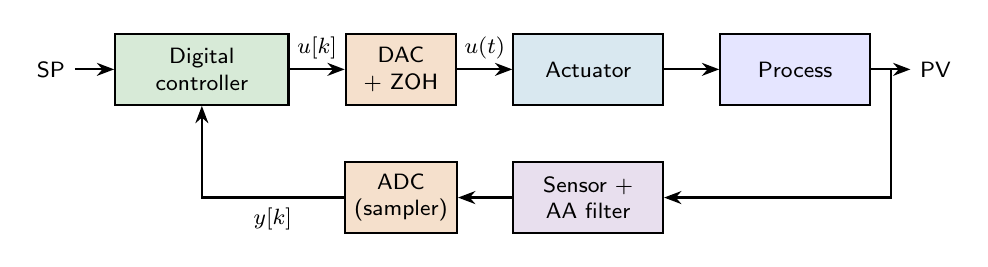
\begin{tikzpicture}[font=\footnotesize, node distance=0.7cm]
					\node (r) {SP};
					\node[blk, right=0.5cm of r, fill=cGreen!18, minimum width=2.2cm] (c) {Digital\\ controller};
					\node[blk, right=of c, fill=cOrange!20, minimum width=1.4cm] (dac) {DAC\\ + ZOH};
					\node[blk, right=of dac, fill=cAccent!15] (a) {Actuator};
					\node[blk, right=of a, fill=blue!10] (p) {Process};
					\node[right=0.5cm of p] (y) {PV};
					\node[blk, below=0.7cm of dac, fill=cOrange!20, minimum width=1.4cm] (adc) {ADC\\ (sampler)};
					\node[blk, below=0.7cm of a, fill=cPurple!15] (s) {Sensor +\\ AA filter};
					\draw[sig] (r) -- (c);
					\draw[sig] (c) -- node[above] {$u[k]$} (dac);
					\draw[sig] (dac) -- node[above] {$u(t)$} (a);
					\draw[sig] (a) -- (p);
					\draw[sig] (p) -- coordinate[pos=0.5] (tap) (y);
					\draw[sig] (tap) |- (s);
					\draw[sig] (s) -- (adc);
					\draw[sig] (adc) -| node[pos=0.25, below] {$y[k]$} (c);
				\end{tikzpicture}
			\end{center}
			\begin{itemize}[itemsep=1pt]
				\item \textbf{Sensor + anti-aliasing (AA) filter} --- measures PV and removes frequencies above $f_s/2$.
				\item \textbf{ADC (sampler)} --- converts PV to a number $y[k]$ every $T$ seconds.
				\item \textbf{Digital controller} --- a CPU running the control algorithm (filter, PID, limits).
				\item \textbf{DAC + zero-order hold} --- converts $u[k]$ to an analog signal and holds it constant until the next sample (``staircase'' output).
				\item \textbf{Actuator \& process} --- as in any control loop.
			\end{itemize}

			\textbf{(b) Sampling and quantisation}
			\begin{itemize}[itemsep=1pt]
				\item \textbf{Sampling}: the controller sees the process only at $t = kT$. Sample at $f_s > 2f_{\max}$ (Nyquist) to avoid \textbf{aliasing}.
				\item \textbf{Quantisation}: an $n$-bit ADC has step $q = \text{FSR}/2^n$ (12-bit, 0--10 V $\Rightarrow$ 2.44 mV); finer resolution needs more bits.
				\item \textbf{Choice of $T$}: $T \le \tau/10$ ($\tau$ = dominant time constant) or 10--20 samples per rise time. Too large $T$ adds delay and can destabilise the loop; too small $T$ wastes CPU time and amplifies noise in the D term.
			\end{itemize}

			\noindent\begin{minipage}[t]{0.52\linewidth}
				\textbf{(c) Implementation flowchart}
				\begin{center}
					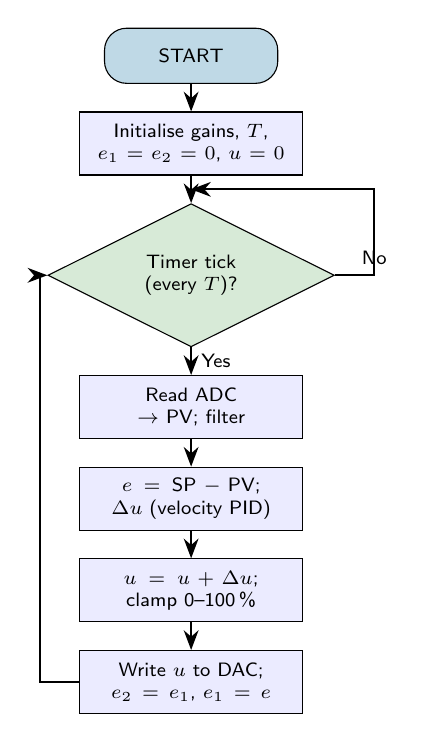
\begin{tikzpicture}[font=\scriptsize, node distance=0.35cm]
						\node[startstop] (st) {START};
						\node[process, below=of st] (in) {Initialise gains, $T$, $e_1 = e_2 = 0$, $u = 0$};
						\node[decision, below=of in] (tk) {Timer tick (every $T$)?};
						\node[process, below=of tk] (rd) {Read ADC $\rightarrow$ PV; filter};
						\node[process, below=of rd] (pid) {$e = \text{SP} - \text{PV}$; $\Delta u$ (velocity PID)};
						\node[process, below=of pid] (cl) {$u = u + \Delta u$; clamp 0--100\,\%};
						\node[process, below=of cl] (wr) {Write $u$ to DAC; $e_2 = e_1$, $e_1 = e$};
						\draw[flowarrow] (st) -- (in); \draw[flowarrow] (in) -- (tk);
						\draw[flowarrow] (tk) -- node[right] {Yes} (rd);
						\draw[flowarrow] (tk.east) -- ++(0.5,0) node[above] {No} |- ($(in.south)!0.5!(tk.north)$);
						\draw[flowarrow] (rd) -- (pid); \draw[flowarrow] (pid) -- (cl); \draw[flowarrow] (cl) -- (wr);
						\draw[flowarrow] (wr.west) -- ++(-0.5,0) |- (tk.west);
					\end{tikzpicture}
				\end{center}
			\end{minipage}\hfill
			\begin{minipage}[t]{0.45\linewidth}
				\textbf{Explanation}
				\begin{itemize}[itemsep=1pt]
					\item A \textbf{hardware timer interrupt} starts each cycle so that $T$ is constant (no jitter from program length).
					\item The measurement is read and \textbf{filtered}: $y_f[k] = a\,y_f[k-1] + (1-a)\,x[k]$.
					\item The \textbf{velocity-form PID} computes only the change $\Delta u$; clamping $u$ provides anti-windup.
					\item The output is written, past errors are shifted, and the controller waits for the next tick.
					\item A \textbf{watchdog} resets the controller if a cycle is not completed in time.
				\end{itemize}
			\end{minipage}
		\end{answer}

		% -------------------------------------------------------------
		\item With a block diagram, explain the architecture of a Programmable Logic Controller. Explain the PLC scan cycle and its response time. Draw a ladder diagram for a motor start/stop circuit with seal-in. \qmarks{10}
		\begin{answer}
			\textbf{(a) PLC architecture}
			\begin{center}
				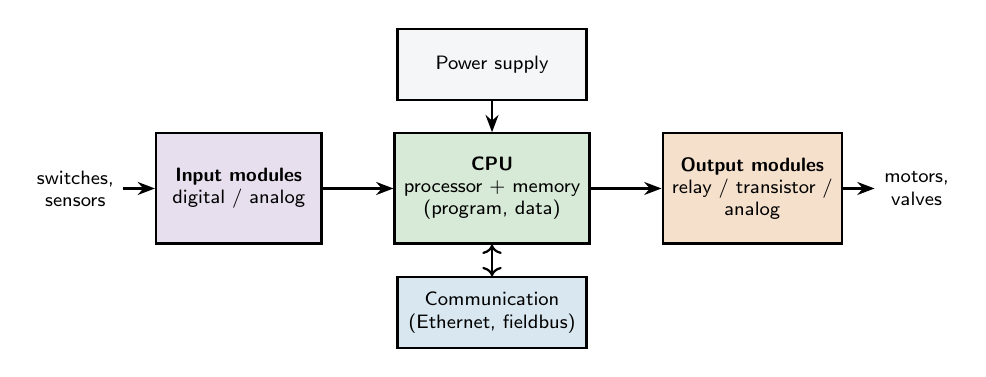
\begin{tikzpicture}[font=\scriptsize, node distance=0.5cm]
					\node[blk, fill=cGreen!18, minimum width=2.4cm, minimum height=1.4cm] (cpu) {\textbf{CPU}\\ processor + memory\\ (program, data)};
					\node[blk, left=0.9cm of cpu, fill=cPurple!15, minimum width=2.1cm, minimum height=1.4cm] (in) {\textbf{Input modules}\\ digital / analog};
					\node[blk, right=0.9cm of cpu, fill=cOrange!20, minimum width=2.1cm, minimum height=1.4cm] (out) {\textbf{Output modules}\\ relay / transistor /\\ analog};
					\node[blk, above=0.4cm of cpu, fill=cGrayBg, minimum width=2.4cm] (ps) {Power supply};
					\node[blk, below=0.4cm of cpu, fill=cAccent!15, minimum width=2.4cm] (com) {Communication\\ (Ethernet, fieldbus)};
					\node[left=0.4cm of in, align=center] (sw) {switches,\\ sensors};
					\node[right=0.4cm of out, align=center] (ld) {motors,\\ valves};
					\draw[sig] (sw) -- (in); \draw[sig] (in) -- (cpu); \draw[sig] (cpu) -- (out); \draw[sig] (out) -- (ld);
					\draw[sig] (ps) -- (cpu); \draw[<->, thick] (cpu) -- (com);
				\end{tikzpicture}
			\end{center}
			\begin{itemize}[itemsep=1pt]
				\item \textbf{Input modules} convert field signals (24 V DC, 4--20 mA) to logic levels, with isolation and filtering.
				\item \textbf{CPU} executes the user program stored in memory, holds the input/output image tables, timers and counters.
				\item \textbf{Output modules} drive contactors, solenoid valves, lamps and analog actuators.
				\item \textbf{Power supply} and \textbf{communication} modules (programming PC, HMI, SCADA, remote I/O).
			\end{itemize}

			\noindent\begin{minipage}[t]{0.40\linewidth}
				\textbf{(b) Scan cycle}
				\begin{center}
					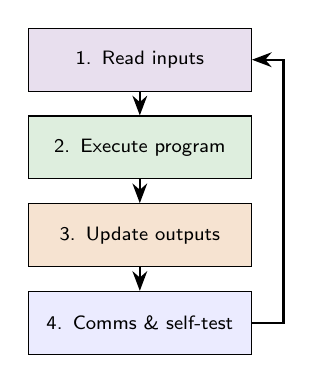
\begin{tikzpicture}[font=\scriptsize, node distance=0.3cm]
						\node[process, fill=cPurple!15] (r) {1. Read inputs};
						\node[process, fill=cGreen!15, below=of r] (e) {2. Execute program};
						\node[process, fill=cOrange!18, below=of e] (w) {3. Update outputs};
						\node[process, fill=blue!8, below=of w] (h) {4. Comms \& self-test};
						\draw[flowarrow] (r) -- (e); \draw[flowarrow] (e) -- (w); \draw[flowarrow] (w) -- (h);
						\draw[flowarrow] (h.east) -- ++(0.4,0) |- (r.east);
					\end{tikzpicture}
				\end{center}
			\end{minipage}\hfill
			\begin{minipage}[t]{0.57\linewidth}
				\textbf{Response time}\\[2pt]
				The scan repeats every 1--50 ms. An input that changes just after being read is only seen in the next scan, so the worst case is
				\[
				t_{\text{resp}} \approx t_{\text{in}} + 2\,t_{\text{scan}} + t_{\text{out}}
				\]
				e.g.\ input filter 3 ms, scan 5 ms, relay output 10 ms $\Rightarrow$ $3 + 10 + 10 = \mathbf{23\ ms}$.
			\end{minipage}

			\medskip
			\textbf{(c) Motor start/stop ladder diagram}
			\begin{center}
				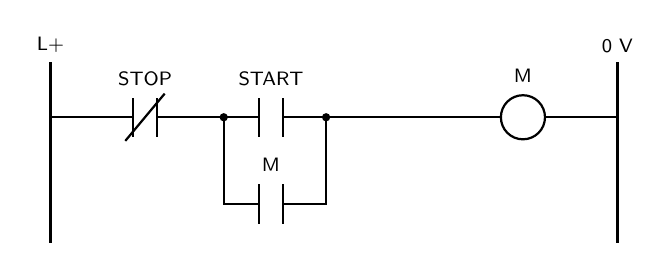
\begin{tikzpicture}[font=\scriptsize]
					\draw[very thick] (0,0.7) -- (0,-1.6);
					\draw[very thick] (7.2,0.7) -- (7.2,-1.6);
					\node[above] at (0,0.7) {L+}; \node[above] at (7.2,0.7) {0 V};
					\draw[thick] (0,0) -- (1.05,0);
					\ladNC{1.2}{0}{STOP}
					\draw[thick] (1.35,0) -- (2.65,0);
					\ladNO{2.8}{0}{START}
					\draw[thick] (2.95,0) -- (5.72,0);
					\ladCoil{6.0}{0}{M}
					\draw[thick] (6.28,0) -- (7.2,0);
					\draw[thick] (2.2,0) -- (2.2,-1.1) -- (2.65,-1.1);
					\ladNO{2.8}{-1.1}{M}
					\draw[thick] (2.95,-1.1) -- (3.5,-1.1) -- (3.5,0);
					\fill (2.2,0) circle (1.5pt); \fill (3.5,0) circle (1.5pt);
				\end{tikzpicture}
			\end{center}
			Pressing \textbf{START} energises coil \textbf{M}; the parallel \textbf{M} contact \emph{seals in} so the motor keeps running after START is released. Pressing \textbf{STOP} (normally closed) breaks the rung and M drops out. After a power failure M stays off (no automatic restart). Equivalent Boolean expression: $M = (\text{START} + M)\cdot\overline{\text{STOP}}$.
		\end{answer}

		% -------------------------------------------------------------
		\item Explain the architecture and functions of a SCADA system with a neat diagram. Compare SCADA with DCS and PLC systems, and list good practices for alarm management. \qmarks{10}
		\begin{answer}
			\textbf{(a) SCADA architecture}
			\begin{center}
				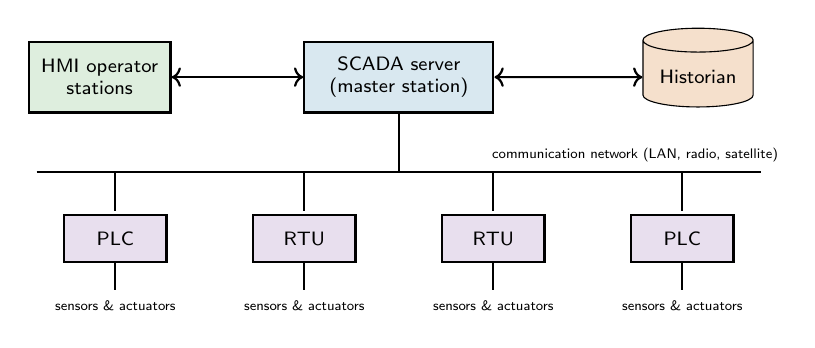
\begin{tikzpicture}[font=\scriptsize]
					\node[blk, fill=cAccent!15, minimum width=2.4cm] (ms) at (0,2.6) {SCADA server\\ (master station)};
					\node[blk, fill=cGreen!15, minimum width=1.8cm] (hmi) at (-3.8,2.6) {HMI operator\\ stations};
					\node[cylinder, draw=black, shape border rotate=90, aspect=0.25, minimum width=1.4cm, minimum height=1.0cm, fill=cOrange!20, align=center] (hist) at (3.8,2.6) {Historian};
					\draw[<->, thick] (hmi) -- (ms); \draw[<->, thick] (ms) -- (hist);
					\draw[thick] (-4.6,1.4) -- (4.6,1.4);
					\node[above, font=\tiny] at (3.0,1.4) {communication network (LAN, radio, satellite)};
					\draw[thick] (ms) -- (0,1.4);
					\foreach \x/\n in {-3.6/PLC, -1.2/RTU, 1.2/RTU, 3.6/PLC} {
						\draw[thick] (\x,1.4) -- (\x,0.9);
						\node[blk, fill=cPurple!15, minimum width=1.3cm, minimum height=0.6cm] at (\x,0.55) {\n};
						\draw[thick] (\x,0.25) -- (\x,-0.1);
						\node[font=\tiny] at (\x,-0.3) {sensors \& actuators};
					}
				\end{tikzpicture}
			\end{center}
			\begin{itemize}[itemsep=1pt]
				\item \textbf{Field devices} --- sensors and actuators on the process.
				\item \textbf{RTUs / PLCs} --- collect field data, run local control, send data on request.
				\item \textbf{Communication network} --- links remote sites to the master (Ethernet, radio, GSM, satellite).
				\item \textbf{Master station} --- polls the RTUs, processes data, runs supervisory logic.
				\item \textbf{HMI} --- mimic diagrams, alarms, trends, operator commands.
				\item \textbf{Historian} --- long-term database for reports and analysis.
			\end{itemize}
			\textbf{Functions}: data acquisition, monitoring, supervisory control (set points, start/stop), alarm handling, trending, reporting, event logging.

			\textbf{(b) Comparison}
			\begin{center}
				\small
				\begin{tabular}{@{}p{2.5cm}p{3.6cm}p{3.6cm}p{4.0cm}@{}}
					\toprule
					\textbf{Feature} & \textbf{PLC} & \textbf{DCS} & \textbf{SCADA} \\
					\midrule
					Main job      & fast logic, machines   & continuous process control & supervision over wide areas \\
					Area          & one machine / cell     & one plant                  & pipelines, grids, fleets \\
					Control loops & some PID               & hundreds of PID loops      & mostly in RTUs / PLCs \\
					Example       & packaging line         & refinery, power plant      & water network \\
					\bottomrule
				\end{tabular}
			\end{center}

			\textbf{(c) Alarm management good practice (ISA-18.2 / EEMUA 191)}
			\begin{itemize}[itemsep=1pt]
				\item Every alarm must require a defined \textbf{operator action}; otherwise make it an event, not an alarm.
				\item \textbf{Prioritise} alarms (critical, high, medium, low) and show priority by colour/sound.
				\item Avoid \textbf{alarm floods}: target less than about one alarm per 10 minutes in normal operation.
				\item Use \textbf{dead-bands} and on/off delays to stop chattering alarms; suppress consequential alarms.
				\item Review alarm statistics regularly and remove nuisance alarms.
			\end{itemize}
		\end{answer}

	\end{enumerate}

\end{document}
